\documentclass{sigchi}

% Use this command to override the default ACM copyright statement (e.g. for preprints).
% Consult the conference website for the camera-ready copyright statement.

%% BEGIN === COPYRIGHT STRIP FOR INITIAL SUBMISSION === Comment In Final Submission
\toappear{{\emph{MOCO'16}}, July 5--6, 2016, Thessaloniki, Greece.}
%% END   === COPYRIGHT STRIP FOR INITIAL SUBMISSION

%% BEGIN === COPYRIGHT STRIP FOR FINAL SUBMISSION === Override in Final Submission
% \toappear{Permission to make digital or hard copies of all or part of this work for personal or classroom use is 	granted without fee provided that copies are not made or distributed for profit or commercial advantage and that copies bear this notice and the full citation on the first page. Copyrights for components of this work owned by others than ACM must be honored. Abstracting with credit is permitted. To copy otherwise, or republish, to post on servers or to redistribute to lists, requires prior specific permission and/or a fee. Request permissions from permissions@acm.org. \\
% Copyright \copyright~2015 ACM ISBN/14/04...\$15.00. \\
% DOI string from ACM form confirmation}
%% END   === COPYRIGHT STRIP FOR FINAL SUBMISSION


% Arabic page numbers for submission.
% Remove this line to eliminate page numbers for the camera ready copy
% \pagenumbering{arabic}


% Load basic packages
\usepackage{balance}  % to better equalize the last page
\usepackage{graphics} % for EPS, load graphicx instead
\usepackage{times}    % comment if you want LaTeX's default font
\usepackage{url}      % llt: nicely formatted URLs
\usepackage{float}    % To allow forcing figure position

% llt: Define a global style for URLs, rather that the default one
\makeatletter
\def\url@leostyle{%
  \@ifundefined{selectfont}{\def\UrlFont{\sf}}{\def\UrlFont{\small\bf\ttfamily}}}
\makeatother
\urlstyle{leo}


% To make various LaTeX processors do the right thing with page size.
\def\pprw{8.5in}
\def\pprh{11in}
\special{papersize=\pprw,\pprh}
\setlength{\paperwidth}{\pprw}
\setlength{\paperheight}{\pprh}
\setlength{\pdfpagewidth}{\pprw}
\setlength{\pdfpageheight}{\pprh}

% Make sure hyperref comes last of your loaded packages,
% to give it a fighting chance of not being over-written,
% since its job is to redefine many LaTeX commands.
\usepackage[pdftex]{hyperref}
\hypersetup{
pdftitle={Movement Of Things Exploring Inertial Motion Sensing When Autonomous, Tiny and Wireless},
pdfauthor={A. Schlegel & C. Honnet},
pdfkeywords={motion, movement data, motion sensing extensions,
    interactive object, embodied interaction, abstract
    visualization},
bookmarksnumbered,
pdfstartview={FitH},
colorlinks,
citecolor=black,
filecolor=black,
linkcolor=black,
urlcolor=black,
breaklinks=true,
}

% create a shortcut to typeset table headings
\newcommand\tabhead[1]{\small\textbf{#1}}


% End of preamble. Here it comes the document.
\begin{document}

\title{Movement Of Things\\
Exploring Inertial Motion Sensing\\
When Autonomous, Tiny and Wireless}

\numberofauthors{2}
\author{
  \alignauthor Andreas Schlegel\\
    \affaddr{LASALLE College of the Arts (Media Lab)}\\
    \affaddr{1 McNally Street, Singapore 187940}\\
    \email{andreas.schlegel@lasalle.edu.sg}\\
  \alignauthor Cedric Honnet\\
    \affaddr{Tangible Display Laboratory}\\
    \affaddr{14 rue des Epernons, 93100 Montreuil, France}\\
    \email{honnet@telecom-paristech.org}\\
}

\maketitle

\begin{abstract}
The Movement of Things project is an exploration into
the qualities and properties of movement. Through a
range of exercises these movements are captured and
translated by custom-built software and the use of an
autonomous, tiny and wireless motion sensor. A series
of Motion Sensing Extensions suggest different
approaches of how to use a motion sensor within
various physical environments to capture movement to
better understand the materialization of movement and
new forms of interactions through movement.
\end{abstract}

\keywords{
	motion; movement data; motion sensing extensions;
    interactive object; embodied interaction; abstract
    visualization
}

\category{H.5.m.}
{Information Interfaces and Presentation (e.g. HCI)}
{Miscellaneous}

\section{Introduction}

The Movement of Things project captures data that can
be measured from the movement of everyday objects.
Here an autonomous, tiny and wireless motion sensor
is attached to a range of custom-built physical
extensions (Fig. 1) to record acceleration and orientation of an
object in various situations.

\begin{figure}[H]
\centering
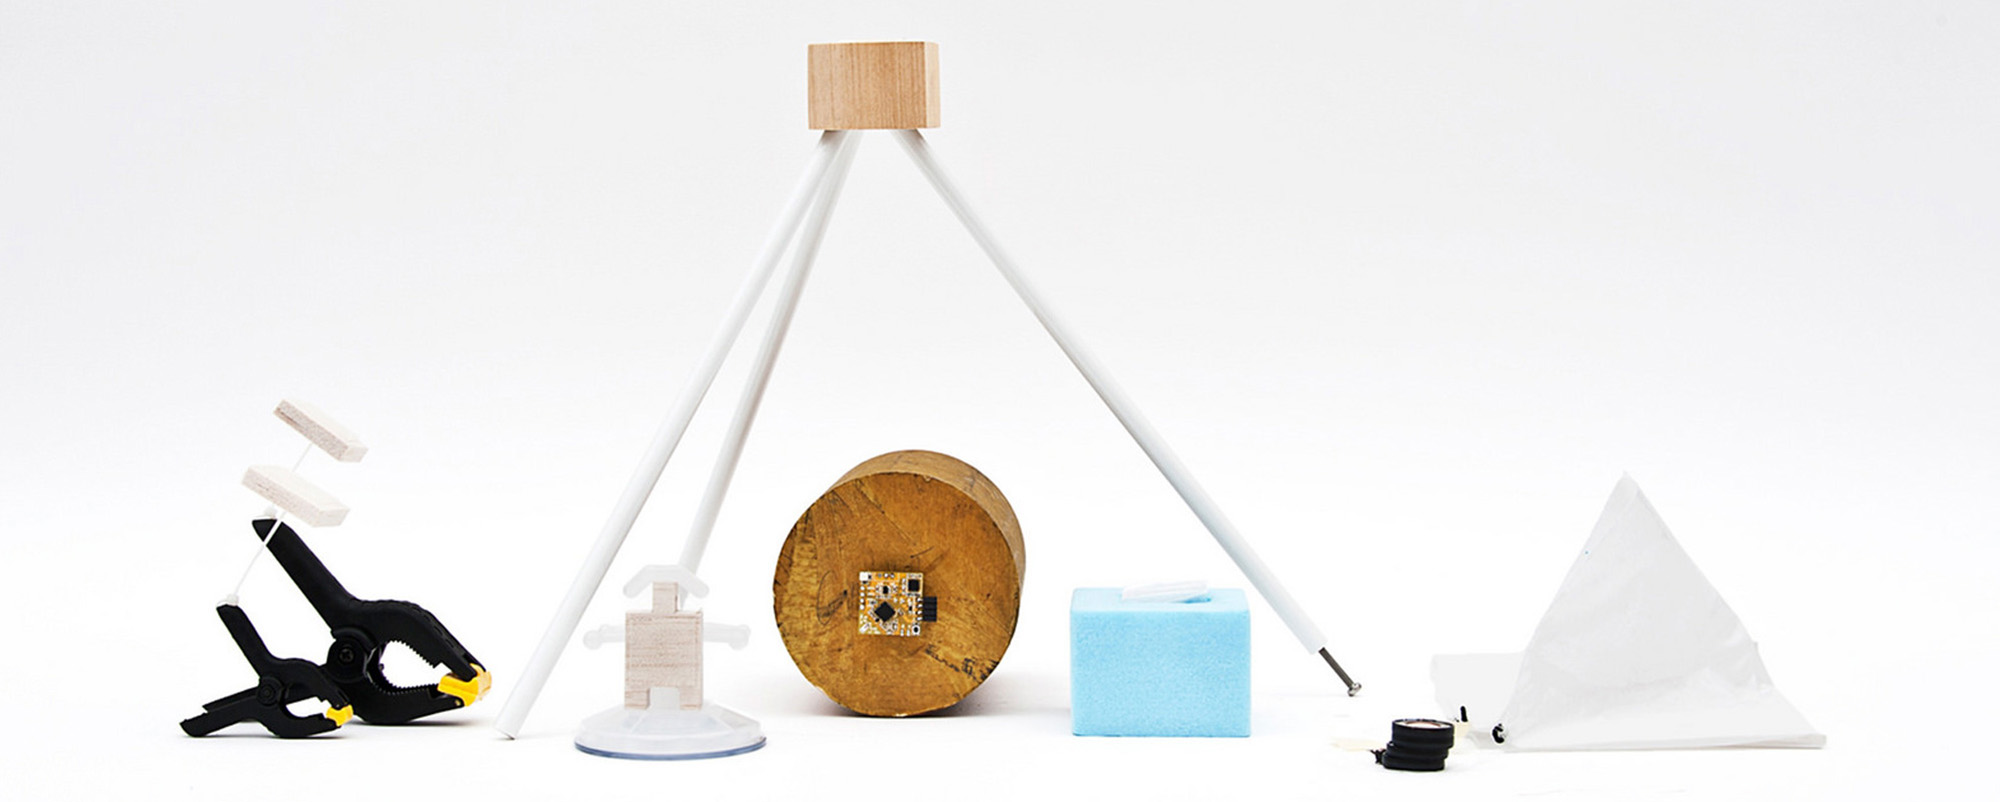
\includegraphics[width=\columnwidth]{pics/extensions}
\caption{Motion Sensing Extensions.}
\label{fig:extensions}
\end{figure}

The transmitted data is
then expressed through an audio or visual medium in
real time or as a recording for further evaluation. With
the Internet of Things at our doorsteps, this project
aims to comment on the increasing ubiquitousness of
sensing technologies in our everyday lives and practices
through performance, play and exploration.
Furthermore we are investigating the potential of
motion data sensors within the arts as a real-time
interface for expressive interactions. How can we
perceive and capture our surroundings through the
lenses of sensing technologies, data and art?

\section{Capturing Movement}

This project makes use of a wireless motion sensor
called the Twiz\cite{twiz}. In order to capture various types of
movement, a range of Motion Sensing Extensions were
built including for example a clamp which can be
attached to a branch of a tree to capture the movement
of the wind swaying through the leaves, a block of
foam to allow the Twiz to float on the surface of water
or a cylindrical shaped piece of plastic to roll the Twiz
along different types of surfaces (Fig. 2).

\begin{figure}[H]
\centering
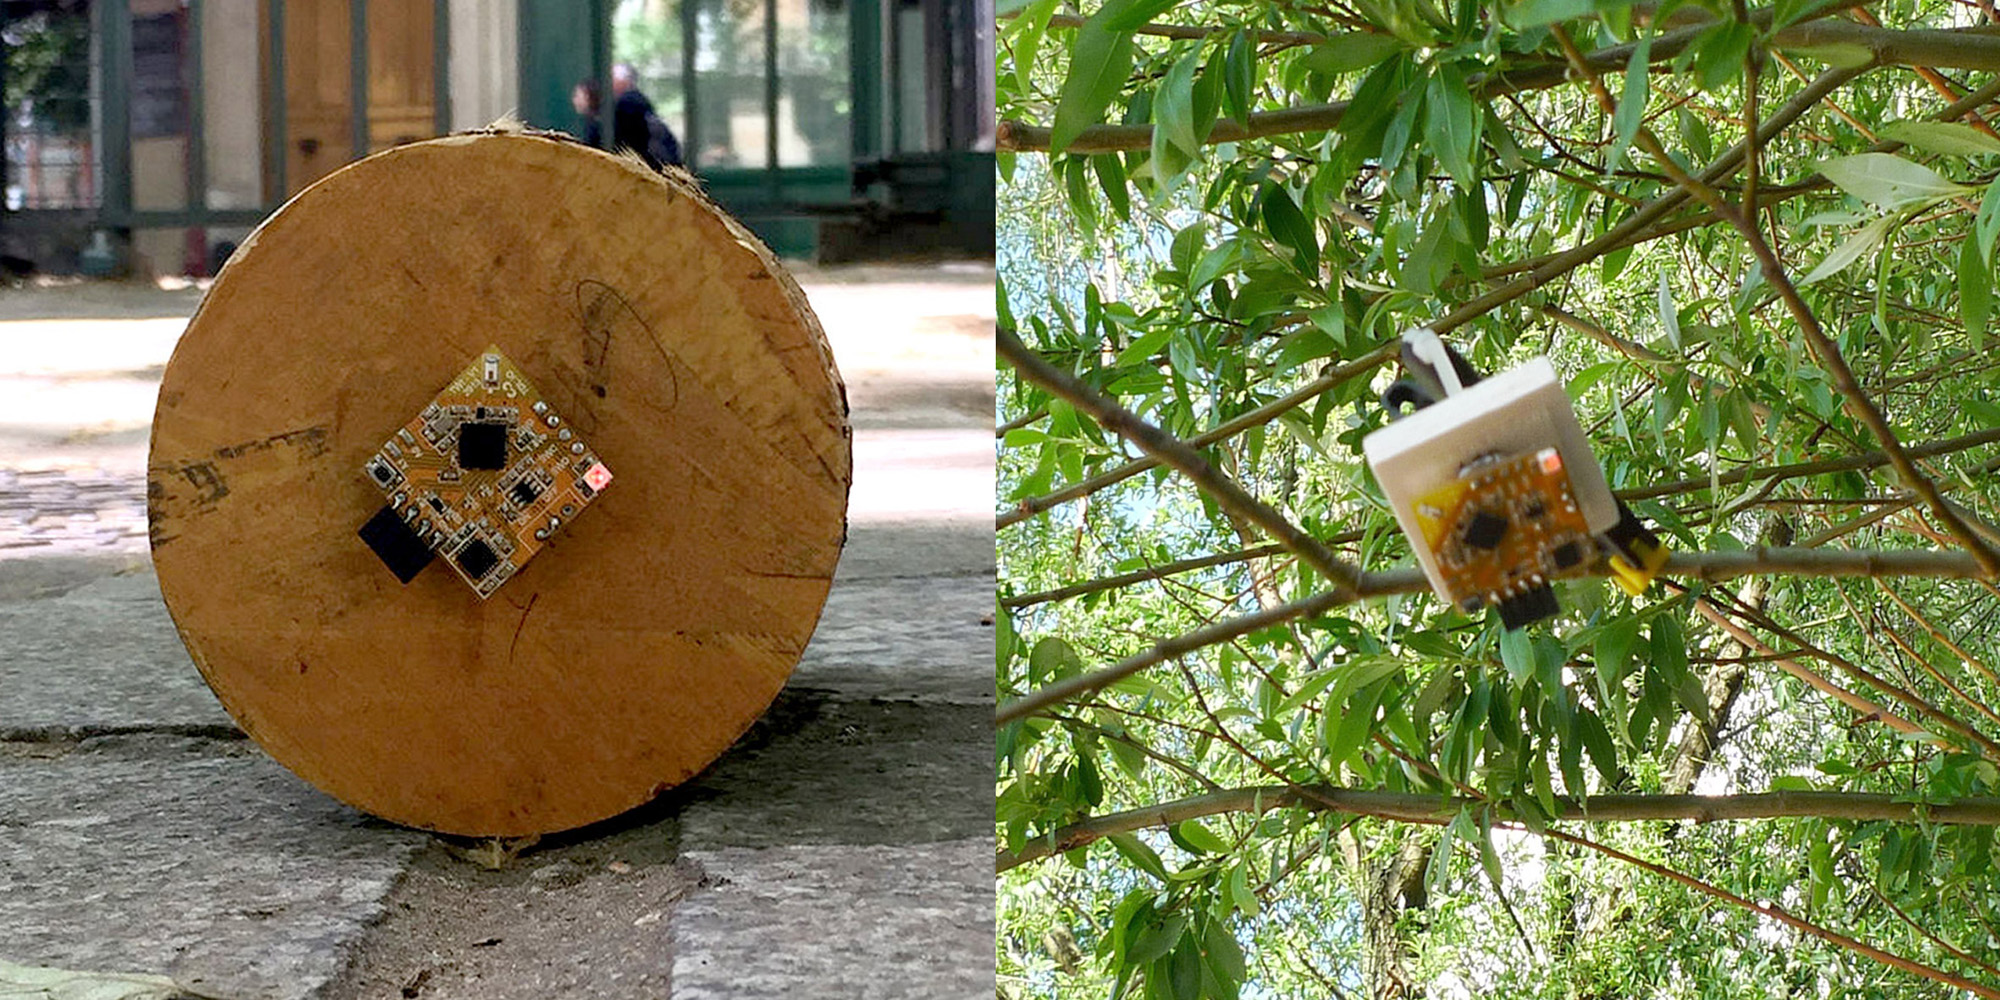
\includegraphics[width=\columnwidth]{pics/fieldtrip}
\caption{The Twiz motion sensor mounted onto a Motion
Sensing Extension (left), and attached to the branch of
a tree to capture the movement of the wind swaying through
the leaves (right).}
\label{fig:fieldtrip}
\end{figure}

\section{Autonomous, Tiny, Wireless Technology}

Different 9 Degrees of Freedom Inertial Measurement Units
(IMU) exist, S. Madgwick\cite {madgwick} developed an
efficient sensor fusion but his hardware was not compact
enough for most use cases and an extra module was needed
to add wireless connectivity.
On a more commercial side, the Hot Hand\footnote
{\url{http://sourceaudio.net/products/hothand}} has the compactness
and autonomy but it only has a 3D accelerometer and the
connectivity is limited.
Then was made the Twiz, the Tiny Wireless IMU, as an open
source project that gathers three 3D inertial sensors
(accelerometer, gyroscope and magnetometer).
A fusion of the sensors data is performed on board.
It uses and adaptation of Madgwick algorithm to
merge the stability of the magnetometer and the
dynamism of the gyroscope. After being processed, this
data is broadcasted wirelessly using a Bluetooth Low
Energy (BLE) advertising hack that uses manufacturer
data, which simplifies the reception as it avoids
connection, and allows multiple listeners. This makes it
easy to communicate with a mobile device to interpret
and record data. Its small size, which is slightly larger
than a coin cell battery, and no-wires-attached
property, allow for much flexibility in use and
application.
The size and flexibility of the Twiz encouraged
experimentation and play in between art and
technology. There was for example the usage of the
first Twiz prototypes to control musical effects. This
gained interest amongst peers over time. This first tiny
version started at noisebridge\footnote{Noisebridge is a
hackerspace for technical-creative projects}, as a collaborative
side project and was improved in many hackerspaces all
around the globe during the hacker trip to china\footnote
{\url{http://noisebridge.net/wiki/NoisebridgeChinaTrip4}}.
This international hackerspaces development allowed a
multi-crowdsourcing feedback, bringing a cultural
cross-pollination and resulted in amazingly enriching
collaborations such as this one.

\section{Interface}

The Movement of Things interface consists of two parts
where the Twiz serves as the data capturing client and a
BLE capable mobile device to record and capture data
within a range of up to 20 meters. The second part
comprises of the so-called Motion Sensing Extensions,
which allow the Twiz to be attached to different objects.
Data is transmitted with an average frame rate of 25
frames per seconds. A custom-built android application
captures and records the data received.

\section{Artistic Expressions}

The objective of the project is to collect the acceleration
and orientation properties of moving objects and
express them artistically. We have tested the
Movement of Things in two different scenarios, a
recorded and a real-time scenario.

\begin{figure}[H]
\centering
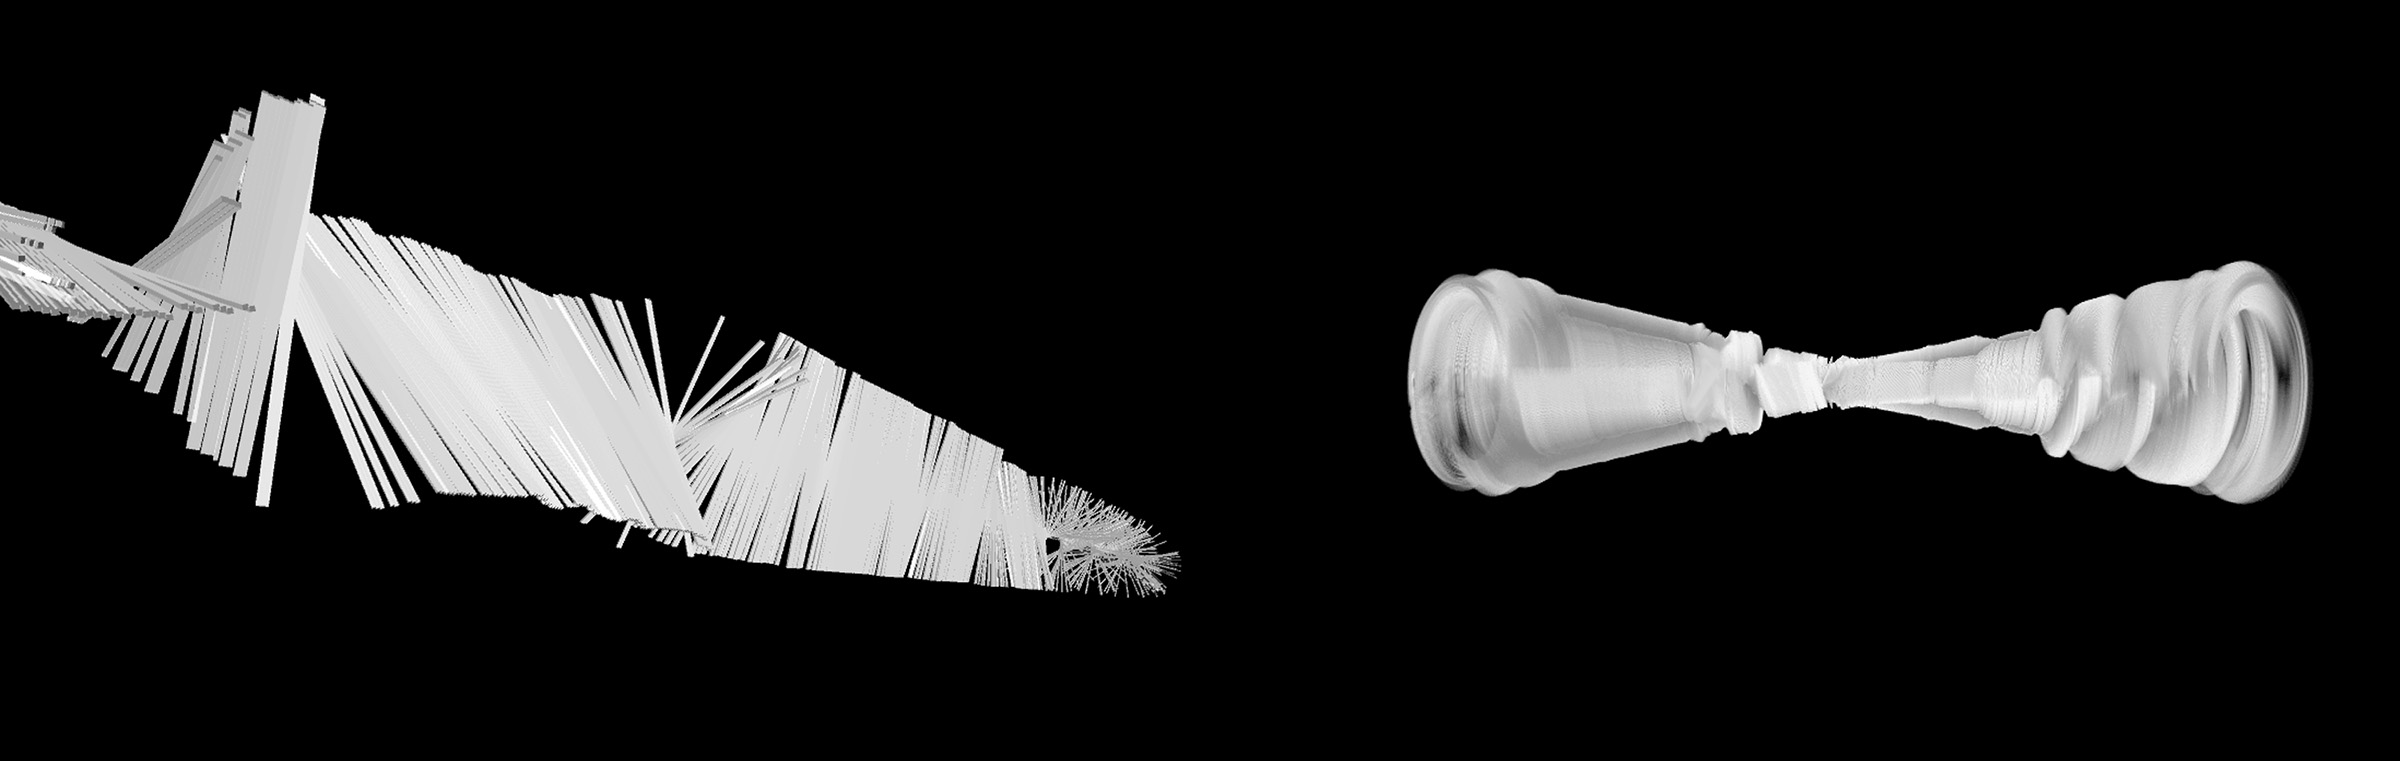
\includegraphics[width=\columnwidth]{pics/renderings}
\caption{Abstract data renderings using data recordings
captured with the Twiz motion sensor.}
\label{fig:renderings}
\end{figure}

\subsection{Recording Scenario}
The recorded scenario took place in May 2015 in Paris
where various subjects found in an urban environment
were measured, including an air vent, washing
machine, dryer, escalator, trees, water, doors or the
metro. Later, the data was interpreted
through abstract data renderings and translated into a
kinetic object animated by data recordings (Fig. 3).



\subsection{Real-time Scenario}
The real-time scenario comprised of a dance
performance presented in August 2015 in Singapore
where dancers would interact with two objects to
respond to and inform an audio-visual system. The
duration of the performance was kept at 10 minutes
and was performed over 30 times, from which
observations of a change in and adaptation of the
dancers interaction with technology can be made. Here
the initial discomfort continuously evolved into a better
understanding of the medium and its improvisational
qualities. For this performance we used Twiz with a glowing
sphere for dancers to carry and perform, and a
suspended wooden bar for dancers to interact with
(Fig. 4). Each object responded with
an audio-visual feedback based on the motion
measured to materialize movement \cite{hansen} through
custom-built software.

\begin{figure}[H]
\centering
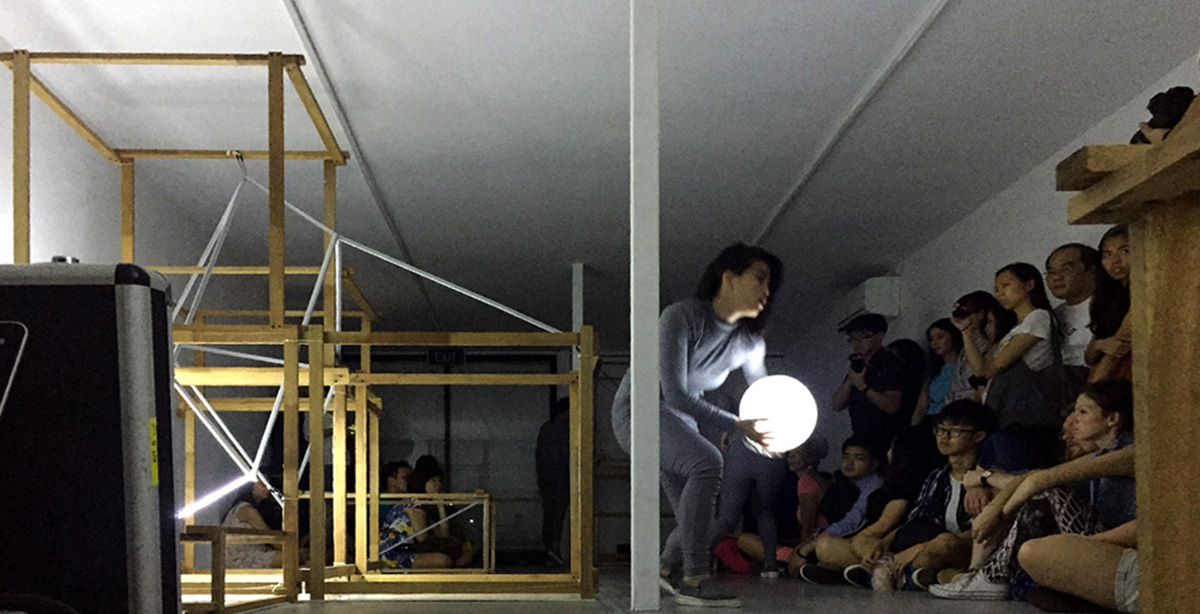
\includegraphics[width=\columnwidth]{pics/performance}
\caption{A dancer holding an object equipped with a Twiz to
interact with the light and sound responsive stage design.}
\label{fig:performance}
\end{figure}

\section{Conclusion}

At this stage of the project, there is an initial
understanding of how to use autonomous, tiny and
wireless motion sensors to sense and measure the
movement of objects under certain conditions. These
had been done within different environments in order to
create a range of artistic expressions. Based on the
projects undertaken, there had been a development of
two scenarios to better understand art-driven
interactions with the use of technology.
By conducting and observing the outcome of each
scenario, there is an initial understanding of how
interactions with this motion sensing technique evolved
over time and how the limitations and the potential can
inform a range of artistic practices through
performance, play and exploration.

\section{Acknowledgements}

We thank LASALLE College of the Arts Singapore, Tangible
Display Labs and Telecom Paristech for their support.

\balance

\bibliographystyle{unsrt}
\bibliography{references}
\end{document}
